\documentclass[a4paper, 11pt]{article}

%set margins
\usepackage[left=2.5cm, top=2.5cm, right=2.5cm, bottom=2.5cm]{geometry}

%package for equations
\usepackage{amsmath}

%package to create directory trees
\usepackage{dirtree}

%package to make hyperlinks from all references
\usepackage[hidelinks]{hyperref}

% disables indentation
\parindent=0pt 

%set space between two paragraphs
\setlength{\parskip}{1em}

%package for figures
\usepackage{graphicx}
\graphicspath{ {../figures/} 
 			   {../icon/} }

%package for captions
\usepackage{caption}

\title{\bf{Kantool behaviour}}
\author{Ir. Maarten Perneel}
\date{\today}


\begin{document}

\maketitle
\thispagestyle{empty}

\begin{figure}[h]
	\centering
	\includegraphics[width=8cm]{Kantool_behaviour_icon}
\end{figure}

\newpage

\tableofcontents
\newpage

\section{Introduction}
The Kantool behaviour application was developed to facilitate keypoint and behaviour annotation. Much focus was placed on generalisability and annotation efficiency, without compromising user-friendliness. In this document, al aspects of the application are elaborately explained.

\section{Application interface}
The main interface of the application is presented in figure \ref{fig:application_main_view}. In this main interface, three parts can be distinguished: the annotation frame, the skeleton frame and the object frame. The size of the frames can easily be adapted to the preferences of the user by moving the sashes between frames. At the left side, one can see the annotation frame, in this frame all annotations are made.

\begin{figure}[htb]
	\centering
	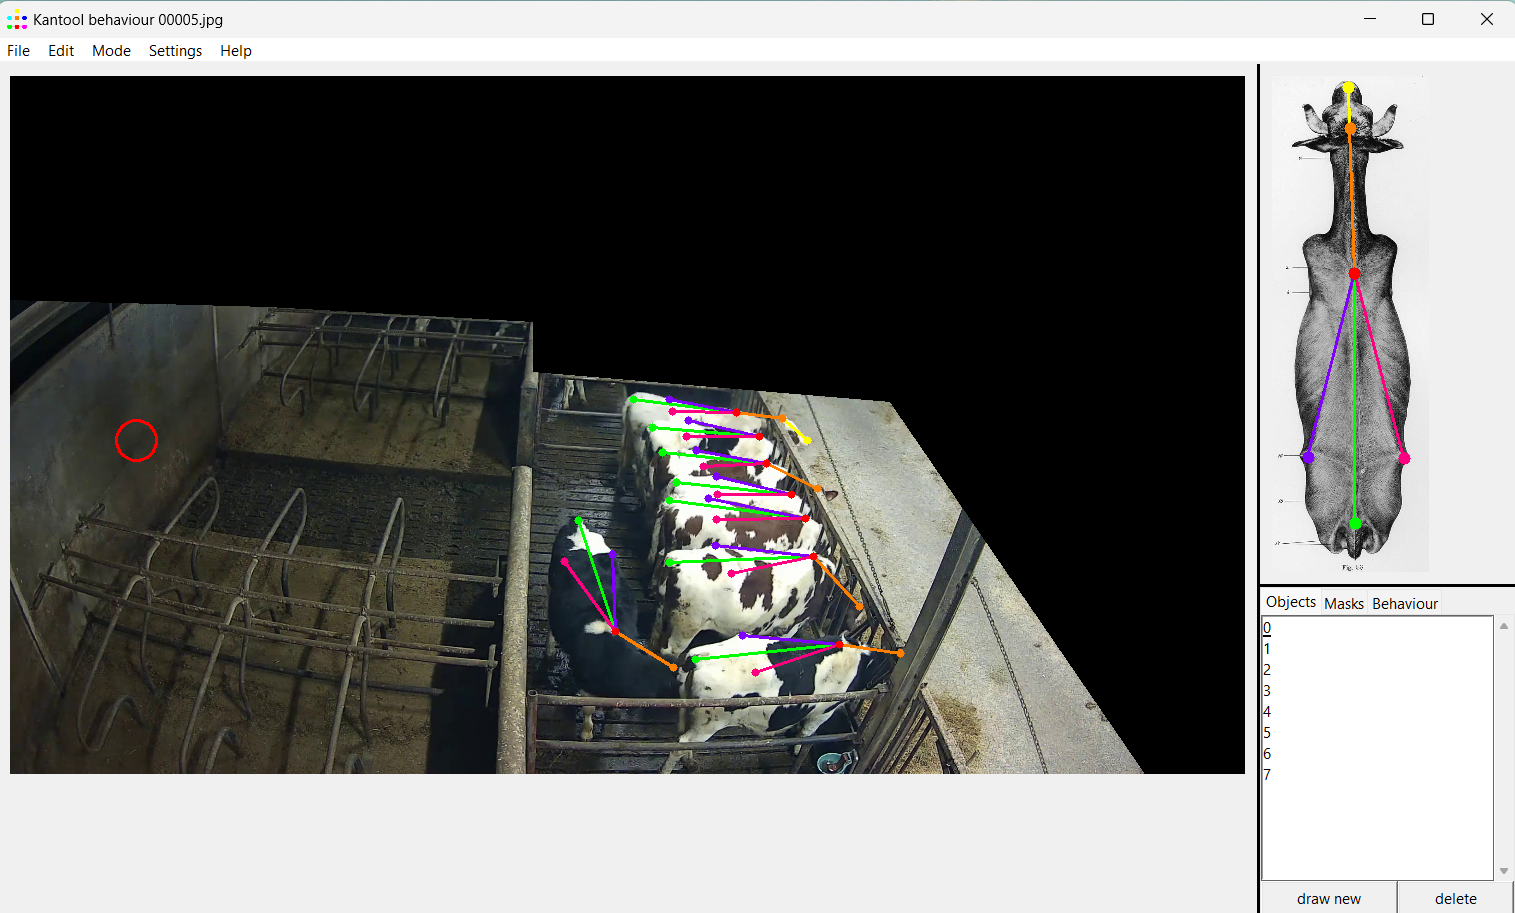
\includegraphics[width=\textwidth]{application_main_view}
	\captionsetup{width=\textwidth}
	\caption{Main interface of the application.}
	\label{fig:application_main_view}
\end{figure}

At the right top part of the application, one can see the skeleton frame, which gives an overview of the skeleton according to which one is making annotations. This skeleton can be imported from previous projects, but can easily be constructed from scratch or adapted by the user. The application offers the possibility to highlight the keypoint that should next be annotated on the skeleton, which allows the user to cope with large skeletons in which it is difficult to purely based on colour derive the current keypoint category. 

Lastly, at the left bottom of the application, one finds the object frame, which lists all annotated objects, masks and behaviours. Masks allow to black out parts of images when this seems necessary to the user. After a skeleton instance was annotated on the image, the application allows to select te respective behaviour of the respective instance.

\section{project outline}
Annotations are always made within projects. A project has a single, unique skeleton and collects all images and annotations in a folder like structure, easily accessible by the user (Figure \ref{fig:project_dir_tree}). The name of the main folder of a project defines the project name. Within this folder, all data and annotations are stored. For each present image (.jpg or .png), a single annotation file is present: "$<$image$>$.json" which contains all keypoint coordinates, instances' behaviours and coordinates of the masks' vertices

\begin{figure}[htb]
	\centering
	\begin{minipage}{5cm}	
		\dirtree{%
			.1 project\textunderscore name.
			.2 project.
			.3 skeleton.jpg.
			.3 skeleton.json.
			.3 ethogram.json.
			.3 mask\textunderscore templates.json.			
			.2 image1.jpg.
			.2 image1.json.
			.2 image2.jpg.
			.2 image2.json.
			.2 ....
		}
	\end{minipage}
	\caption{Directory tree of a project}
	\label{fig:project_dir_tree}
\end{figure}

Next to these files, also the folder "project" can be found, which stores all project specifications. The file "skeleton.json" within this folder stores all skeleton specifications, while  "skeleton.jpg" or "skeleton.png", which contains a background image to facilitate the interpretation of the skeleton. Additionally, there is also a file "ethogram.json", which stores the ethogram definition.  Next to these obligatory files, also the facultative file "mask\textunderscore templates.json" can be present, which stores mask templates, stored by the user to apply them generically on multiple images.

\section{Create a new project}
When the application is started, the user has the option to open a project or to create a new project via the file menu. When the user wants to open a yet existing project (Ctrl+Shift+O), the main folder of the project should be selected ("project\textunderscore name" in Figure \ref{fig:project_dir_tree}). When a new project should be initiated (Ctrl+Shift+N), a wizard will pop up to guide the user during the project initiation. When finished, this wizard will create the directory tree specified in Figure \ref{fig:project_dir_tree}.

\begin{figure}[htb]
	\centering
	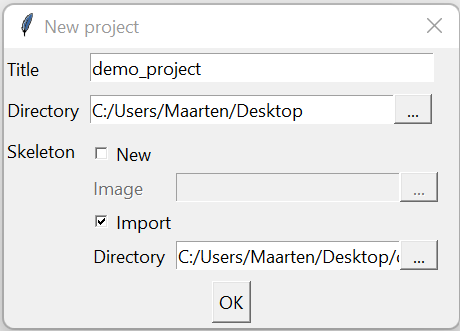
\includegraphics[width=0.5\textwidth]{new_project_wizard}
	\captionsetup{width=0.5\textwidth}
	\caption{Wizard to create a new project.}
	\label{fig:new_project_wizard}	
\end{figure}

When creating a new project, the user has the option to create a new project, in this case, only an appropriate background image (.png or .jpg) should be selected. Alternatively, the user can opt to reuse a skeleton from a previous project, in this case, the "project" folder of a yet existing project (Figure \ref{fig:project_dir_tree}) should be specified. When the user opted to reuse a yet existing skeleton architecture, the application will be in annotation mode after the wizard finished (Figure \ref{fig:application_main_view}) and the user can immediately start to import images. On the other hand, if the user wants to define a new skeleton architecture, the application will be in skeleton mode (Figure \ref{fig:application_skeleton_mode}) once the wizard finished and the user can easily define the new skeleton

\section{Create and modify the skeleton architecture}
To create or modify the skeleton architecture, the application should first be in skeleton mode (Figure \ref{fig:application_skeleton_mode}). Remark the background of the application becomes red when in skeleton mode, since wrong adaptations to the skeleton can lead to severe and permanent data loss. To define a new keypoint, one can click the left mouse button at the appropriate location on the skeleton background image. This will activate a pop up in which one can specify the name, parent and color of a keypoint.

\begin{figure}[htb]
	\centering
	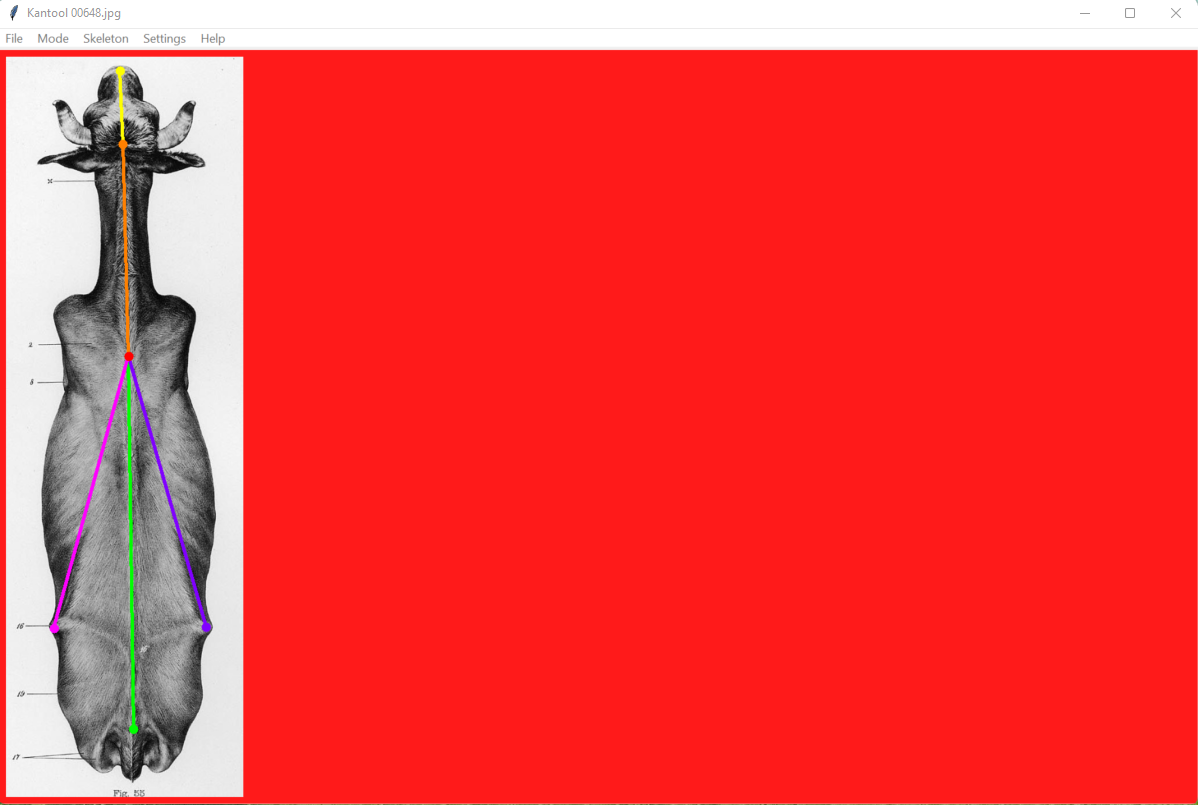
\includegraphics[width=\textwidth]{application_skeleton_mode}
	\captionsetup{width=\textwidth}
	\caption{Skeleton mode of the application}
	\label{fig:application_skeleton_mode}	
\end{figure}

The skeleton architecture should be hierarchically in order to be valid. This means that, except from the central keypoint, each keypoint should have one and only one parent keypoint to which it is connected. When initiating a skeleton, this central keypoint is the first keypoint that is drawn, however, the central keypoint can easily be changed later on via Skeleton $>$ Change central keypoint.

All properties of keypoints can be modified after initial declaration. To move a keypoint, one can simply re-activate the keypoint by clicking , moving the keypoint to the desired location and releasing again the left mouse button. To change other properties of a keypoint, one can double click on a keypoint, after which the keypoint properties dialog will pop up again.

\section{Mask Templates}
It often happens the same masks have to be drawn on multiple consecutive images. In order to facilitate this task, the mask template manager can be used. After drawing the mask template (consisting out of multiple masks), one can save a mask template via Edit $>$ Save mask template. After specifying the name of the template, the mask template will be saved and available for generic application. To apply a saved mask template on an image, one can import the mask template via Edit $>$ Import mask template. Remark that importing a mask template won't delete previously declared masks and multiple mask templates can be consecutively imported for a single image. If the user is importing images into the project, the application will by default ask for a mask template to apply on all of the imported images.

\section{Added features}

\subsection{Name masks}
The application allows to name masks, this can be done by double clicking on the masks automatically generated name in the object frame, after which one can specify a new name for the mask

\subsection{Magnetic borders}
When drawing a mask, often mask vertices should be drawn on the edges of the image. Since this is often not straightforward, the borders of the image in the annotation frame are made magnetic. If one tries to declare a new mask vertex within this magnetic border, the vertex will automatically be placed onto the image border. The magnetic borders are only active when declaring a new mask vertex, when one is moving a mask vertex by dragging the vertex while holding the left mouse key, the magnetic borders are not active and therefore allow to place a mask vertex within the magnetic border, but not on an edge of the image. The magnetic borders are by default 40 px wide, but their wideness can be modified via Settings.

\section{Mouse events}

\begin{tabular}{ p{3cm} p{14cm}}
	left click & Draw a new point. If one clicks on a yet existing point, the point will be re-activated and can be moved to a more appropriate position. If one clicks on an edge of a mask, the edge will be splitted and a new point will appear on the place were one clicked. One can move the active point as long as one holds down the left mouse button. Once the left mouse button is released, the point will be fixed on it's current position\\
	right click & When annotating an object, the right mouse button allows to skip a keypoint, if the keypoint of that category is not visible for the object that's one currently annotating. When a keypoint was re-activated, clicking the right mouse button will de-activate the keypoint and one can complete the annotations for the selected object (if the object was incomplete)\\
	scroll & Zoom in/out \\  
	scroll wheel click & Move the image (only available if the image doesn't fit on the window)     
\end{tabular}


\section{Shortcuts}

\begin{tabular}{ll}
	Enter & Confirm object\\
	Del & Delete point\\
	Ctrl + Del & Delete object/delete mask\\
	Ctrl + Shift + O & Open project\\
	Ctrl + Shift + N & New project\\
	Ctrl + O & Open image\\  
	Ctrl + W & Close image\\  
	Ctrl + S & Save annotations\\ 
	Ctrl + I & Import images\\
	F1 & Open help\\ 
	F5 & Export dataset\\ 
	F7 & Open previous image\\ 
	F8 & Open next image\\  
\end{tabular}

\end{document}